

%----------------------------------------------------------------------------------------
% 			I. PREFACE AREA OF THE DOCUMENT
%----------------------------------------------------------------------------------------

\documentclass[12p]{article}

\usepackage{graphicx}
\graphicspath{ {images/} }

%----------------------------------------------------------------------------------------
% 			 II.  BEGIN OF THE DOCUMENT
%----------------------------------------------------------------------------------------


\begin{document}


%----------------------------------------------------------------------------------------
%			  PAGE 1 : TITLE PAGE
%----------------------------------------------------------------------------------------

\begin{titlepage}

\pagenumbering{gobble}		% Delete the page number for the title page

\newcommand{\HRule}{\rule{\linewidth}{0.5mm}} % Defines a new command for the horizontal lines, change thickness here

\center % Center everything on the page
 
%----------------------------------------------------------------------------------------
%			Heading Section of the title
%----------------------------------------------------------------------------------------

\textsc{\Huge University of Helsinki}\\[2cm] % Name of your university/college
\textsc{\LARGE Computer Science Department}\\[0.5cm] % Major heading such as course name

%----------------------------------------------------------------------------------------
%				Title section
%----------------------------------------------------------------------------------------

\HRule \\[0.4cm]
{ \Huge \bfseries PreAssignment 2016}\\[0.4cm] % Set the title of the document
\HRule \\[2.5cm]
 

%----------------------------------------------------------------------------------------
%				Author Section
%----------------------------------------------------------------------------------------

% If you don't want a supervisor, uncomment the two lines below and remove the section above
\LARGE \emph{Author:}\\
\LARGE Andres Medina\\[0.05cm] % Your name
\textsc{\Large (UAF 1608168)}\\[3cm] % Your name

%----------------------------------------------------------------------------------------
%				Date Section
%----------------------------------------------------------------------------------------

{\LARGE \today}\\[3cm] % Date, change the \today to a set date if you want to be precise

 
%----------------------------------------------------------------------------------------

\vfill % Fill the rest of the page with whitespace

\end{titlepage}


%----------------------------------------------------------------------------------------
%				END OF THE TITLE PAGE
%----------------------------------------------------------------------------------------


  \newpage 				% Creates a new page


%----------------------------------------------------------------------------------------
%				PAGE 2:  	TABLE OF CONTENTS
%----------------------------------------------------------------------------------------

  \tableofcontents 			% Creates the table of contents page



  \newpage 				% Creates a new page


%----------------------------------------------------------------------------------------
%				PAGE 3:  	TASK 1
%----------------------------------------------------------------------------------------


  \pagenumbering{arabic}		% Restores the page number (could also be used with roman for roman numbers)


%----------------------------------------------------------------------------------------
%				Title section
%----------------------------------------------------------------------------------------

\begin{center}

  \textsc{\LARGE Preassignment - Task 1}\\[1cm] % Title of the second page

\end{center}

%----------------------------------------------------------------------------------------
%				(1) First section
%----------------------------------------------------------------------------------------
 
  \section{Introduction}			% Subsection of a document

%   First Paragraph
  \large The first task of the preassignment consists in experimentally test that the amortized complexity of $(n-1)$ calls to \textbf {inorder\_next} in a binary tree is $2(x-1)$.

\bigskip

%   Second Paragraph
 \large To achieve this task, the following strategy was followed:

\begin{enumerate}

  \item First, we created a program that generates random Binary Trees. This allows us to had a test set in which we prove the current hypothesis.
  \item After creating the random Binary Tree generator, we create a second program that allows us to transverse the binary tree in inorder \textit{(inorder means, first visiting the left node, then the root and finally the right node)}. The program also returns the amount of steps involved in this operation.
  \item By using both programs, we made a table that compare the amount of steps taken to transverse every binary tree in comparison with the number of nodes of each tree.
  \item Finally, we made a plot with the data of the table and by using linear regression, we get the equation corresponding to that line plot. We expect that the slope of that line plot should be something bigger or equal to $2(x-1)$ \textit{(it should be bigger or equal because the amortized complexity correspond to an upper bound of the actual complexity of an algorithm)}.

\bigskip

The results obtained in the analysis are described in the results section of this paper.

\end{enumerate}


%----------------------------------------------------------------------------------------
%				(2) Second section
%----------------------------------------------------------------------------------------

  \section{Materials and Methods}
In this section, we will describe the tools and the logic used to solve every single step that composed the task 1 of this preassignment. This section include topics like the programming framework used to solve this task and also what was the logic applied to develop those programs.


%----------------------------------------------------------------------------------------
%				(2.1) First Subsection
%----------------------------------------------------------------------------------------

  \subsection{Programming Tools}
For developing the required programs we choose to use the following tools:

\begin{itemize}
  \item Python 3.5.1 as the programming language
  \item Github as a repository tool
  \item Sublime Text as the code editor
\end{itemize}

In addition, the random library of python was used for accomplish the tasks related with randomness.


%----------------------------------------------------------------------------------------
%				(2.2) Second Subsection
%----------------------------------------------------------------------------------------

  \subsection{Programming Logic}
The two programs involved in this task were programmed by using OOP paradigm.
Considering the fact that the task 1 of the preassignment involves the creation of two different programs, we choose to explain the logic of each program in a different subsection. 


  \subsubsection{Creating a Random Binary Tree}

The creation of the binary tree was implemented by developing two different classes: a binary node class and a binary tree class. The binary node class contains 3 different attributes, an Id, a reference to a left child node and a reference to a right child node while the binary tree class contains only two attributes, a list of binary nodes and the total cost of traversing the tree in inorder. By using this two classes, creating a random binary tree was possible. Also when every binary tree is created, a random tree setting method is called so that every tree created has a different and also random structure.

\bigskip

The random tree setting method work as follows: 
\begin{itemize}
  \item First, a  integer number between 50 and 100 is choose randomly. This number will represent the number of nodes of the corresponding binary tree
  \item Second, a left-right flag is set by choosing a random integer number between 0 and 1
  \item Then, after the left-right flag is set, a random node of the tree is chosen. Only the nodes that doesn't already have the corresponding child are candidates for this random choice. \textit{For example, if the left-right flag is set to left, only nodes that doesn't have left childs are possible candidates of this random choice. Conversely, if the left-right flag is set to right, only nodes that doesn't have right childs are possible candidates}
  \item Finally, the corresponding child is created in the randomly chosen node of the tree
\end{itemize}

The described logic repeats until the number of nodes of the binary tree is reached.

  \subsubsection{Traversing a Binary Tree in inorder}
The traversing of a binary tree in inorder can be made mainly in two different ways: by using recursion and by not using recursion. In this case, we choose to implement this method using recursion as this method allow to achieve a smaller and cleaner code and also allow us to avoid the implementation of a link between a child node and it's parent node.

\bigskip

The idea of this implementation is mainly the following:
\begin{itemize}
  \item We start by applying this method to the root node of the tree
  \item If the root node has a left child, then we call again the traverse\_inorder method but this time we pass the left child node as an argument to the method
  \item When the corresponding node has no left child node, then we ask if the node has a right child. If the node has a right child, then we call again the traverse\_inorder method but this time we pass the right child node as an argument to the method
  \item After no more left and right child are found, the traverse\_inorder method returns. Of course we should consider a logic for counting the corresponding steps in each call of the method so that when the method ends, we have the total amount of steps already calculated.
\end{itemize}

In the next section we will show and analyze the results of the above implementations.

%----------------------------------------------------------------------------------------
%				(3) Third section
%----------------------------------------------------------------------------------------

  \section{Results}
When the two generated programs are run, an output table is created. This table includes three columns:
\begin{enumerate}
  \item \textbf{Binary Tree ID } Represents the Id of the binary tree
  \item \textbf{Number of nodes of the Tree } Represents the number of nodes of the binary tree 
  \item \textbf{Total steps of inorder traverse } Represents the amounts of steps involved in the inorder traverse operation
\end{enumerate}

The results obtained in this computation are shown in the following table:

%----------------------------------------------------------------------------------------
%				Table section
%----------------------------------------------------------------------------------------

\footnotesize
\begin{table}[ht]
\caption{Binary Tree traverse results using 50 different trees}	% title of Table
%\centering 									% used for centering table
\begin{tabular}{c c c} 							% centered columns (3 columns)
\hline\hline 									%inserts double horizontal lines
Tree Id & Number of Nodes & Total Steps\\ [0.5ex] 			% inserts table
%heading
\hline % inserts single horizontal line
1 & 83 & 164 \\ 								% inserting body of the table
2 & 94 & 186 \\
3 & 69 & 136 \\
4 & 99 & 196 \\
5 & 53 & 104 \\
6 & 63 & 124 \\
7 & 72 & 142 \\
8 & 61 & 120 \\
9 & 55 & 108 \\
10 & 90 & 178 \\
11 & 81 & 160 \\
12 & 74 & 146 \\
13 & 92 & 182 \\
14 & 85 & 168 \\
15 & 75 & 148 \\
16 & 66 & 130 \\
17 & 95 & 188 \\
18 & 64 & 126 \\
19 & 71 & 140 \\
20 & 95 & 188 \\
21 & 52 & 102 \\
22 & 77 & 152 \\
23 & 53 & 104 \\
24 & 84 & 166 \\
25 & 80 & 158 \\
\hline %inserts single line
\end{tabular}
\qquad
%\centering 									% used for centering table
\begin{tabular}{c c c} 							% centered columns (3 columns)
\hline\hline 									%inserts double horizontal lines
Tree Id & Number of Nodes & Total Steps\\ [0.5ex] 			% inserts table
%heading
\hline % inserts single horizontal line
26 & 70 & 138 \\
27 & 95 & 188 \\
28 & 68 & 134 \\
29 & 88 & 174 \\
30 & 98 & 194 \\
31 & 99 & 196 \\
32 & 63 & 124 \\
33 & 66 & 130 \\
34 & 59 & 116 \\
35 & 94 & 186 \\
36 & 85 & 168 \\
37 & 59 & 116 \\
38 & 68 & 134 \\
39 & 93 & 184 \\
40 & 62 & 122 \\
41 & 75 & 148 \\
42 & 100 & 198 \\
43 & 92 & 182 \\
44 & 82 & 162 \\
45 & 84 & 166 \\
46 & 58 & 114 \\
47 & 63 & 124 \\
48 & 69 & 136 \\
49 & 51 & 100 \\
50 & 66 & 130 \\ 
\hline %inserts single line
\end{tabular}

\label{table:nonlin} % is used to refer this table in the text
\end{table}

  \newpage 				% Creates a new page

\large By inspecting the results of the table we can clearly see that the amount of steps that takes to traverse a binary tree, directly depends of the amount of nodes that compose that particular binary tree. 

\bigskip

To obtain the equation that describes the relation between the number of nodes and the amount of steps that takes to traverse a binary tree, we decided to plot the data in the table shown previously and use linear regression to obtain the equation. The result of this linear plot is shown in the following image:

%----------------------------------------------------------------------------------------
%				Graph section
%----------------------------------------------------------------------------------------

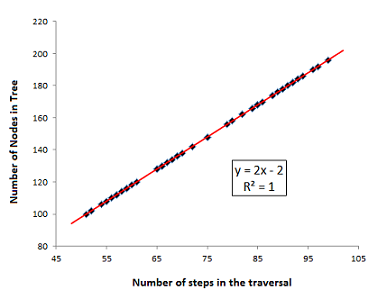
\includegraphics{Graph2}

As we can see, the value of the \textbf{coefficient of determination} also know as $R^2$ is 1. This means that the linear regression line perfectly fits the plotted data. The equation that describes this relation is correspond to $y=2x-2$ where $x$ represents the number of nodes in a binary tree and $y$ represents the amounts of steps that takes to traverse that particular tree in inorder.

\bigskip

We will discuss the meaning of this result in the next section of the text.

%----------------------------------------------------------------------------------------
%				(3) Forth section
%----------------------------------------------------------------------------------------

  \section{Discussion}

As we saw in the last section, the amount of steps that takes to traverse a random binary tree in inorder is $2x-2$ where $x$ represents the number of nodes of that particular tree. In this section, we will use this result to test experimentally that the amortized complexity of $(n-1)$ calls of \textbf{inorder\_next} correspond to $2(x-1)$.

\bigskip

To do this task, we need to consider the following information:
\begin{itemize}
  \item First, the amortized complexity is an upper bound on total actual complexity. \textit{This means that the amortized complexity is always bigger or equal than the total actual complexity}
  \item Second, the operation of traverse an entire binary tree with $n$ nodes is exactly the same than call the \textbf{inorder\_next} function $n$ times
  \item Third, if we do $n$ calls to a function the actual complexity of this operation will always be bigger or equal than the actual complexity of $n-1$ calls to the same function
\end{itemize}

\bigskip
\bigskip

Using the above information and also considering the results obtained in the last section, we can state the following:
\begin{itemize}
  \item The actual complexity for $n$ calls of \textbf{inorder\_next } can be represented by the equation $2(x-1)$. \textit{where $x$ represents the number of nodes in a binary tree}
  \item Considering that $n-1$ calls to a function is les expensive than $n$ calls in the same function (in terms of complexity), we can state than \textbf{$2(x-1)$ is an upper bound of the actual complexity of $n-1$ calls}. \textit{This state is based in the fact that $2(x-1)$ will always be bigger or equal than the actual complexity of $n-1$ calls}
  \item Finally as $2(x-1)$ is an upper bound of the actual complexity of $n-1$ calls to the function \textbf{inorder\_next}, we can also said that $2(x-1)$ \textbf{is a possible value for the amortized complexity of this function}
\end{itemize}

\bigskip

In conclusion, by collecting data and using the method shown in this paper, we managed to test experimentally that $2(x-1)$ or $2x-2$ is a totally possible value for the amortized complexity of $n-1$ calls of the \textbf{inorder\_next} function.

\end{document}



